\chapter{QED and nuclear corrections}
\addtocontents{toc}{\contentsline{chapter}{QED and nuclear corrections}{\protect\pageref{annotation}}}
\label{ch:Improvements}

This chapter presents the calculation of the leading-order contributions of the most important effects previously neglected in our formulation of the ECM. Specifically, the corrections to bound state energies coming from the Breit interaction, finite-nuclear-size effect and vacuum polarization. The results show good agreement with reference values already in the leading order.  

\section{Relativistic potentials}

The potentials used in our derivation of the ECM and D-ECM were all non-relativistic, that is, of the form~$\frac{1}{r}$. This makes them instantaneous and so a good description only of the interaction with the nucleus (since it is assumed stationary), %(what about magnetic interaction?!)
 but not of the interaction between electrons, when they are moving with relativistic velocities. A more accurate, fully relativistic form of the interaction between two charged particles can be derived using the theory of quantum electrodynamics (QED). The equations describing QED however, cannot be solved exactly, so in practice the resulting corrections have to be treated perturbatively. 
 
 In order to improve the form of the potential, one needs to understand which corrections are most relevant. For this reason let us first examine the scaling of different interactions and their respective corrections. In Schr\"odinger theory the interaction between the electrons and nucleus is proportional to the nuclear charge squared $Z^2$ (see~\eqref{SchrA}), while the first-order interaction between pairs of electrons (see~\eqref{SchrB}) is proportional to $Z$ (in the case of $Z^*=Z$)\footnote{It is conventional to factor out the powers of $Z$ and refer to the relative scaling of the electron-electron interaction to the electron nuclear interaction, as $1/Z$}. The difference between the Schr\"odinger and Dirac descriptions scales to leading order as $(\alpha Z)^2$ (see~\eqref{DiracA}), so we can say that the relativistic corrections are of the order $Z(\alpha Z)^2$. Notice however that, by using the fully relativistic D-ECM wavefunctions we have accounted for the electron-nucleus interactions to all orders in $(\alpha Z)$. 
 
 Interactions in QED are conveniently represented using Feynmann diagrams~\cite{FD}, where the leading-order interactions correspond to the exchange of a single virtual photon. In the case of two electrons, such interaction is described (in the limit of low frequency) by a potential of the form:
 \begin{equation}
     V(r) = \frac{1}{r_{ij}} + B_{ij},
 \end{equation}
 where $B_{ij}$ is an off-diagonal operator of the order $Z(\alpha Z)^2$, called the Breit operator~\cite{bethe2014quantum}. It contains magnetic interaction coming from electron's spin, as well as leading-order retardation effects (both electric and magnetic). A similar correction term can be written for the electron-nucleus interaction, but since we assume the nucleus to be stationary, the is no retardation and only the magnetic effect remains. Both of these are presented in figure~\ref{BreitFig}.

\section{Breit interaction}

Using the Dirac matrices, defined by~\eqref{DiracAlpha}, we can write the Breit operator as~\cite{bethe2014quantum}\footnote{This is the low frequency limit of the Breit operator. The full frequency dependent version - as implemented for example in the GRASP2k package - can be found in~\cite{Si2019CriticalEO}.}
\begin{equation}
B_{ij} = \frac{1}{2}\left(\frac{\vec{\alpha}_i \cdot \vec{\alpha}_j}{|\vec{r}_{ij}|}+\frac{(\vec{\alpha}_i \cdot r_{ij}) (\vec{\alpha}_j \cdot \vec{r}_{ij})}{|\vec{r}_{ij}|^3}\right),
\end{equation}
where the indices~$i,j$ label a pair of electrons, and the inner product runs through the three Dirac matrices~$\vec{\alpha} = (\alpha_1, \alpha_2, \alpha_3)$.

\begin{figure*}
  \centering  
\subfigure{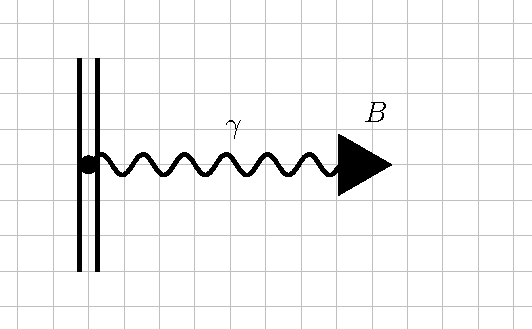
\includegraphics[width=69mm]{Graphs/NucleusBreitMagnetic.pdf}}
 % \hspace{10mm}
    \subfigure{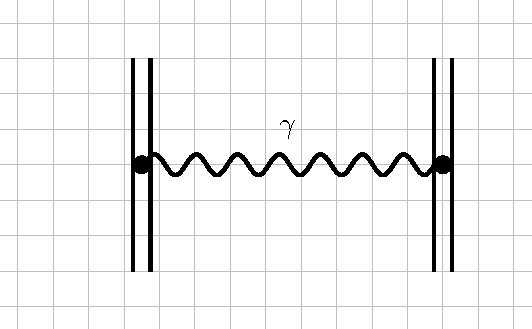
\includegraphics[width=69mm]{Graphs/BreitFeynmanLabeled.pdf}}
  \caption{Feynman diagrams of the leading-order magnetic interaction between an electron and the nucleus (left) and of the Breit interaction between two electrons (right). The double lines represent bound states of electrons in the field of the nucleus. The wiggly line is the photon propagator and triangle represents the interaction with the magnetic field of the nucleus.}
  \label{BreitFig}
\end{figure*}

The operator~$B_{ij}$ contains the $\frac{1}{r_{ij}}$ potential, as well as leading-order retardation effects and the magnetic interaction coming from electron's spin (notice that it involves off-diagonal elements in the standard representation). Similarly there is a magnetic interaction between the spin of the nucleus and that of the electrons, which in the leading order is described by an exchange of a single virtual photon. Both of these presented in figure~\ref{BreitFig}.

Since the two terms in the Breit operator are similar in magnitude~\cite{00018737000101191}, for our purposes we approximate the Breit operator as
\begin{equation}
B_{ij} \approx \frac{\vec{\alpha}_i \cdot \vec{\alpha}_j}{|\vec{r}_{ij}|}.
\end{equation}

We can then apply the Wigner-Eckhart theorem~\cite{sakurai2020modern} to the general case to get
\begin{align}
\langle \lambda_1 \lambda_2 | \frac{\vec{\alpha}_i \cdot \vec{\alpha}_j}{|r_i-r_j|} | \lambda_3 \lambda_4 \rangle &= \sum_i\frac{\langle \lambda_1 | \alpha^i | \lambda_3 \rangle \langle \lambda_2 | \alpha^i | \lambda_4 \rangle}{|r_1-r_2|} \nonumber
\\
&= 2\sum_{p,J} M_{pJ}(\overline{\lambda_3},\lambda_1)M_{pJ}(\lambda_2,\overline{\lambda_4})R_P(g_1 g_2 f_3 f_4) \nonumber
\\
&+2\sum_{p,J} M_{pJ}(\overline{\lambda_3},\lambda_1)M_{pJ}(\overline{\lambda_2},\lambda_4)R_P(g_1 f_2 f_3 g_4) \nonumber
\\
&+2\sum_{p,J} M_{pJ}(\lambda_3,\overline{\lambda_1})M_{pJ}(\lambda_2,\overline{\lambda_4})R_P(f_1 g_2 g_3 f_4) \nonumber
\\
&+2\sum_{p,J} M_{V}(\lambda_3,\overline{\lambda_1})M_{pJ}(\overline{\lambda_2},\lambda_4)R_P(f_1 f_2 g_3 g_4), \label{BreitFull}
\end{align}
with the angular part given by~\cite{PhysRev.154.17}
\begin{align}
M_{Jp}(\lambda_1,\lambda_2) = &\sqrt{3(2l_1+1)(2l_2+1)(2J+1)(2j_1+1)(2j_2+1)} \\
&\times\begin{pmatrix}
j_1 & j_2 & J
\\
-m_1 & m_2 & m_1-m_2
\end{pmatrix}\begin{pmatrix}
l_1 & l_2 & p
\\
0 & 0 & 0
\end{pmatrix}
\left\{\begin{matrix}
l_1 & 1/2 & j_1
\\
l_1 & 1/2 & j_1
\\
k & 1 & k
\end{matrix}\right\},
\end{align}
and the radial by
\begin{equation}
R_p(\psi_1 \psi_2 \psi_3 \psi_4) = \int \psi_1 (r_1) \psi_2 (r_2) \psi_3 (r_1) \psi_4 (r_2) \frac{r_<^p}{r_>^{p+1}}r_1^2r_2^2dr_1 dr_2,
\end{equation}
where the overline indicates a flip of the sign of the relativistic quantum number~$\kappa$.

Like in the Coulomb case, for a two-electron Slater determinant, we get a difference between direct and exchange terms
\begin{equation}
\langle \lambda_1 \lambda_2 | \frac{\vec{\alpha}_i \cdot \vec{\alpha}_j}{|r_i-r_j|} | \lambda_1 \lambda_2 \rangle = \langle \lambda_1 | \langle \lambda_2 | \frac{\vec{\alpha}_i \cdot \vec{\alpha}_j}{|r_i-r_j|} | \lambda_1 \rangle | \lambda_2 \rangle - \langle \lambda_1 | \langle \lambda_2 | \frac{\vec{\alpha}_i \cdot \vec{\alpha}_j}{|r_i-r_j|} | \lambda_2 \rangle | \lambda_1 \rangle,
\end{equation}
while the total contribution to the energy of a multi-electron atom can be written as
\begin{align}
    \langle \lambda_1 ... \lambda_n | \frac{\alpha_1 \cdot \alpha_2}{r_{12}} |\lambda_1 ... \lambda_n \rangle &= \sum_{i < j}^n \langle \lambda_i \lambda_j | \frac{\alpha_1 \cdot \alpha_2}{|r_1-r_2|} |\lambda_i \lambda_j \rangle \nonumber
    \\
    &= \frac{1}{2}\sum_{i,j}^n \langle \lambda_i \lambda_j | \frac{\alpha_1 \cdot \alpha_2}{|r_1-r_2|} |\lambda_i \lambda_j \rangle,
\end{align}
where the final form on the right hand side is most useful for deriving formulas for closed shells. 

Plugging in~\eqref{BreitFull}, we get the direct term as
\begin{equation}
\langle \lambda_1 | \langle \lambda_2 | \frac{\alpha_i \cdot \alpha_j}{|r_i-r_j|} | \lambda_1 \rangle | \lambda_2 \rangle = 8 \sum_p M_{pp}(\lambda_1,\lambda_1)M_{pp}(\lambda_2,\lambda_2)R_p(g_1 g_2 f_1 f_2).
\end{equation}
However since
\begin{equation}
\sum_m \begin{pmatrix} j & j & J\\-m & m & 0 \end{pmatrix} = 0,
\end{equation}
the sum over projections vanishes in this case for any value of~$p$
\begin{equation}
\sum_{m}M_{pp}(\lambda,\lambda)=0,
\end{equation}
so the direct term is zero for a closed shell.
The exchange term on the other hand becomes
\begin{align}
M_{\lambda_1 \lambda_2} = & \langle \lambda_1 | \langle \lambda_2 | \frac{\alpha_i \cdot \alpha_j}{|r_i - r_j|} | \lambda_2 \rangle |\lambda_1 \rangle \nonumber
\\
 = & 2\sum_{p} \big[\epsilon_{p }(\ovjrline{\lambda_1},\lambda_2)R_p(g_1 g_1 f_2 f_2) +\epsilon_{p }(\lambda_1,\overline{\lambda_2})R_p(f_1 f_1 g_2 g_2)2 \nonumber
 \\
 &+ f_{p}(\lambda_1,\lambda_2)R_p(g_1 g_2 f_1 f_2)\big].
\end{align}

\begin{table}[t]
\centering
\begin{tabular}{cc|lllr}
	Element & Z &~$E^{\rm{Br}}_{\rm{D-ECM}}(Z)$ &~$E^{\rm{Br}}_{\rm{D-ECM}}(Z^*)$ & $E^{\rm{Br}}_{\rm{DHF}}$ & $ \Delta E^{\rm{Br}}$\\
	\hline
	\hline 
	He & 2 & 0.00005 & 0.00003 & 0.00006 & 50\% \\
	Be & 4 & 0.00056 & 0.00034 & 0.00071 & 52\%\\
	C & 6 & 0.00571 & 0.00312  & 0.00283 & 10\%\\
	Ne & 10 & 0.0377 & 0.0179 & 0.0175 & 2\%\\
	Mg & 12 & 0.0674 & 0.0334 & 0.0339 & 1\%\\
	Si & 14 & 0.124 & 0.0623 & 0.0588 & 6\%\\
	S & 18 & 0.290 & 0.146 & 0.143 & 2\%\\
	Ar & 20 & 0.404 & 0.209 & 0.208 & 0\%\\
	Zn & 30 & 1.74 & 0.831 & 0.838 & 1\% \\
	Kr & 36 & 3.27 & 1.58 & 1.58 & 0\% \\
	Cd & 48 & 8.73 & 4.25 & 4.28 & 1\% 
	 \\
	\hline
\end{tabular}
	\caption{Comparison of the magnetic Breit correction to the energy of closed-shell neutral atoms between the~$1/Z$ expansion up to first order ($\Delta E^{\rm{Br}}(Z)$), leading-order D-ECM ($\Delta E^{\rm{Br}}(Z^*)$) and a full perturbative solution of the DHF equations ($\Delta E^{\rm{Br}}_{DHF}$). Reference data from~\cite{DESCLAUX1973311}. Last column gives the relative difference between the leading-order D-ECM and DHF results.}
	\label{tab:Breit}
\end{table}

After a trivial summation over~$m_1,m_2$ and a complicated summation over~$J$ we get the coefficients in closed form as
\begin{equation}
f_p(\lambda_1,\lambda_2)=2|\kappa_1 \kappa_2|
\begin{pmatrix} j_1 & j_2 & p \\ -1/2 & 1/2 & 0 \end{pmatrix}^2
\end{equation}
\begin{align}
\epsilon_p(\lambda_1,\lambda_2)=\frac{2|\kappa_1 \kappa_2|}{\kappa_2+1/2}\Big[(\kappa_2-1/2&)
\begin{pmatrix} j_1 & j_2 & p \\ -1/2 & 1/2 & 0 \end{pmatrix}^2 \nonumber
\\
&+2(\kappa_2+1)
\begin{pmatrix} j_1 & |\kappa_2+1|-1/2 & p \\ 1/2 & -1/2 & 0 \end{pmatrix}^2\Big].
\end{align}

The corresponding magnetic correction to the electron-nuclear interaction can be treated in an analogous way and the contribution of the direct term is similarly equal to zero. However, in this case there is no exchange contribution, since the nucleus is a distinguishable particle from the electron. This means there is no Breit correction to the electron-nucleus interaction.

In table~\ref{tab:Breit} we present the leading order ECM calculation of the Breit operator contribution to energy of some closed-shell neutral atoms. We see that the accuracy is of the order of~$1\%$ even for large atoms. % (what about small ones?!)
In calculating the Breit correction, we have used the value of effective charge found for the pure Dirac equation. One could instead include the Breit term in the Hamiltonian to begin with, in order to find a "self-consistent" value of effective charge. However, we found no significant difference in the final result.


\begin{table}[]
    \centering
    \begin{tabular}{ccc|ccc}
	Element & Z &~$r_{RMS}$ &~$\Delta E^{\rm{FNS}}_{1/Z}$ &~$\Delta E^{\rm{FNS}}_{D-ECM}$ & ~$\Delta E^{\rm{FNS}}_{DHF}$ \\
	\hline 
	\hline
	He & 2 & 3.72 $\times 10^{-5}$ & 2.96 $\times 10^{-8}$ & 1.78 $\times 10^{-8}$ & 1.94 $\times 10^{-8}$\\
	Be & 4 & 4.36 $\times 10^{-5}$ & 7.36 $\times 10^{-7}$ & 4.40 $\times 10^{-7}$ & 5.69 $\times 10^{-7}$\\
	C & 6 & 4.67 $\times 10^{-5}$ & 4.31 $\times 10^{-8}$ & 2.35 $\times 10^{-8}$  & 3.59 $\times 10^{-6}$\\
	Ne & 10 & 5.75 $\times 10^{-5}$ & 5.19 $\times 10^{-5}$ & 2.43 $\times 10^{-5}$ & 3.90 $\times 10^{-5}$\\
	Mg & 12 & 5.78 $\times 10^{-5}$ &  1.14 $\times 10^{-4}$ & 5.55 $\times 10^{-5}$  & 9.25 $\times 10^{-5}$\\
	Si & 14 & 6.16 $\times 10^{-5}$ &  2.23 $\times 10^{-4}$ & 1.09 $\times 10^{-4}$  & 1.93 $\times 10^{-4}$\\
	Ar & 18 & 6.33 $\times 10^{-5}$ & 7.47 $\times 10^{-4}$ & 3.59 $\times 10^{-4}$  & 6.88  $\times 10^{-4}$\\
	Zn & 30 & 7.43 $\times 10^{-5}$ & 9.97 $\times 10^{-4}$ & 4.14 $\times 10^{-4}$ & 8.73 $\times 10^{-3}$\\
	Kr & 36 & 7.86 $\times 10^{-5}$ & 2.66 $\times 10^{-2}$ & 1.09 $\times 10^{-2}$ & 2.43 $\times 10^{-2}$\\
	Cd & 48 & 8.47 $\times 10^{-5}$ & 1.40 $\times 10^{-1}$ & 5.12 $\times 10^{-2}$ & 1.27  $\times 10^{-1}$\\
	\hline
    \end{tabular}
	\caption{Finite-nuclear-size corrections to energy of closed-shell neutral atoms calculated with leading-order~D-ECM and with the first-order $1/Z$ expansion compared to results of a DHF calculation. Nuclear radii ($r_{RMS}$) taken from~\cite{ANGELI201369}. Reference data taken from~\cite{VISSCHER1997207}.}
	\label{tab:FNS}
\end{table}

\section{Finite-nuclear-size effect}

Another class of corrections to the energy of atoms are those coming from the properties of the nucleus. So far we have been describing the nucleus, as a point particle which is a good approximation only for small nuclei. For heavier ones, properties like size, shape and magnetic moment can have noticeable contributions to binding energies. In general, the most significant contribution comes from the size of the nucleus~\cite{Valuev_2020}. For this reason, for the purpose of estimating the size of nuclear corrections, we model the nucleus as a uniformly charged sphere
\begin{equation}
\rho(r) = \frac{3 Z}{4 \pi r_0^3}\theta(r_0-r),
\end{equation}
where~$r_0$ is the effective nuclear radius, related to the root-mean-square of the nuclear charge distribution as
\begin{equation}
r_0 = \sqrt{\frac{5}{3}\langle r^2\rangle}.
\end{equation}

This leads to a nuclear potential of the form
\begin{equation} \label{NucCharge}
 V_{\rm{FNS}} =
    \begin{cases}
      r<r_0 & -\frac{Z}{2 r_0}\left(3-\frac{r^2}{r_0^2}\right)\\
      r>r_0 & -\frac{Z}{r}\\
    \end{cases}       
\end{equation}

The correction to total energy is given by the expectation value of the difference between the finite-sized nuclear and point-like nuclear potentials
\begin{equation}
\Delta E_{\rm{FNS}} = \sum_\lambda \langle \lambda | \delta V_{\rm{FNS}}(r)|\lambda \rangle =\sum_\lambda \langle \lambda | V_{\rm{FNS}} + Z/r |\lambda \rangle. %= \int |R_{\lambda} (r)|^2 (V_{FNS}(r)+Z/r)r^2 dr 
\end{equation}

The generating integral of the potential difference can easily be found analytically
\begin{align}
I_q^\lambda (r_0) = \int_0^{\infty} e^{-\lambda r} r^q \delta V_{FNS}(r) &= \int_0^{r_0} e^{-\lambda r} r^q \frac{Z}{2 r_0}\left(\frac{2 r_0}{r}-3+\frac{r^2}{r_0^2}\right) \nonumber
\\
&= \frac{Z}{\lambda^q} \left( \frac{\gamma_{q+3}(\lambda r_0)}{2\lambda^3r_0^3}-\frac{3\gamma_{q+1}(\lambda r_0)}{2\lambda r_0}-\gamma_{q}(\lambda r_0)\right)
\end{align}
where~$\gamma_s(x)$ is the lower incomplete gamma function (see Appendix~\ref{app:Gamma}).

Finally, since hydrogen-like wavefunctions are composed of elementary functions, we can easily calculate the finite-nuclear-size correction for any configuration as a finite sum of~$I_q^\lambda (r_0)$ terms with corresponding powers. %(what is the final formula?!)
 The results for some neutral atoms are presented in table~\ref{tab:FNS}.

\section{Vacuum polarization}

With the Breit operator, we have included all QED corrections to the electron-electron interaction up to the order of~$Z(\alpha Z)^2$, with further corrections being at least of order~$Z(\alpha Z)^3$. There is however a correction to the nuclear-electron interaction that is of the order~$\alpha(\alpha Z)$, %(is it?!)
corresponding to the simplest vacuum polarization diagram, as shown in figure~\ref{UehlingFig}. The contribution of such interaction to the nuclear potential is called the Uehling potential. It has been derived for an arbitrary nuclear charge distribution~$\rho_N$ as~\cite{refId0} 
\begin{equation}
V_{\rm{Ue}}(r) = -\frac{8}{3} \alpha^2\int r'\rho_N(r') \frac{e^{-2t|r-r'|}-e^{-2t(r+r')}}{4rt}\left(1+\frac{1}{2t^2}\right)\frac{\sqrt{1-t^2}}{t^2} dt dr'.
\end{equation}

\begin{figure}  
  \centering
  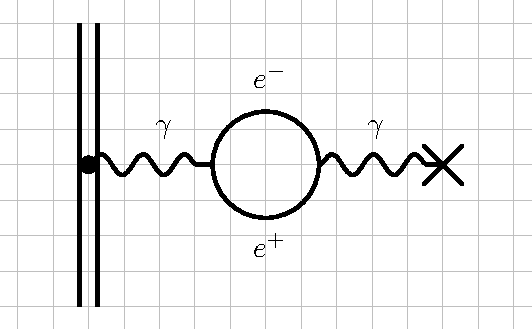
\includegraphics[width=80mm]{Graphs/UehlingLabeled.pdf} 
  \caption{Feynman diagram of the leading-order vacuum polarization contribution to the electron-nucleus interaction. The double lines represent bound states of electrons in the field of the nucleus. Wiggly line is the photon propagator and cross represents the interaction with the field of the nucleus. The double line represents a bound state of the electron and circle a free electron-positron loop.}
  \label{UehlingFig}
\end{figure} 		

Using the charge distribution of~\eqref{NucCharge}, we get the generating integral of the Uehling potential as
\begin{align}
\int e^{-\lambda r}V_{Ue}(r) r^q dr =-\frac{2\alpha^2 Z}{\pi r_0^3}\int e^{-2r_0t}&\big(K_{\lambda,q}(t)+S_{\lambda,q}(t) \nonumber
\\
&-S_{\lambda,q}(-t)\big)\left(1+\frac{1}{2t^2}\right)\frac{\sqrt{1-t^2}}{16 t^5} dt,
\end{align}
and we have defined:
\begin{align}
 S_{\lambda,q}(t) =& (1+2r_0t)\frac{\gamma_q((2t+\lambda)r_0)}{(2t+\lambda)^{q}}, \\ K_{\lambda,q}(t)=&(1+2r_0t+e^{4r_0t}(2r_0t-1))\frac{\Gamma_q((2t+\lambda)r_0)}{(2t+\lambda)^{q}},
\end{align}
where $\gamma_q$ and $\Gamma_g$ are the lower and upper incomplete gamma functions respectively (see Appendix~\ref{app:Gamma}). Closed form of this expression can be found in the limit of small nuclear radius
\begin{align}
I_q^\lambda (r_0) =\int e^{-\lambda r}V_{Ue}(r) r^q dr = -\frac{\alpha^2 Z}{12\pi}(J_{q,1}(\lambda)-\lambda J_{q+1,3}(\lambda)) + O[r_0^2],
\end{align}
where
\begin{align}
J_{q,i}(\lambda) = \Gamma \left(\frac{q}{2}\right)^2\Bigg(\frac{q}{(q+1)(q+3)}&
	{_3F_2}\left[\frac{q}{2},\frac{q+1}{2},\frac{q}{2}+1;\frac{q+5}{2},\frac{i}{2};\frac{\lambda^2}{4}\right] \nonumber
	\\
	&+\frac{2}{q+1}{_3F_2}\left[\frac{q}{2},\frac{q+1}{2},\frac{q}{2};\frac{q+3}{2},\frac{i}{2};\frac{\lambda^2}{4}\right]\Bigg),
\end{align}
and ${}_3F_2$ are the generalized hypergeometric functions.

\begin{table}[]
    \centering
    \begin{tabular}{ccc|cc}
	Element & Z &~$r_{RMS}$ &~$\Delta E^{\rm{Ue}}_{1/Z}$ &~$\Delta E^{\rm{Ue}}_{D-ECM}$ \\
	\hline 
	\hline
	He & 2 & 3.72 $\times 10^{-5}$ & 3.42 $\times 10^{-5}$ & 2.39 $\times 10^{-5}$ \\
	Be & 4 & 4.36 $\times 10^{-5}$ & 2.92 $\times 10^{-4}$ & 2.13 $\times 10^{-4}$ \\
	C & 6 & 4.67 $\times 10^{-5}$ & 9.37 $\times 10^{-4}$ & 6.55 $\times 10^{-4}$ \\
	Ne & 10 & 5.75 $\times 10^{-5}$ & 4.12 $\times 10^{-3}$ & 2.69 $\times 10^{-3}$ \\
	Mg & 12 & 5.78 $\times 10^{-5}$ &  6.89 $\times 10^{-3}$ & 4.64 $\times 10^{-3}$ \\
	Si & 14 & 6.16 $\times 10^{-5}$ &  1.05 $\times 10^{-2}$ & 7.18 $\times 10^{-3}$  \\
	Ar & 18 & 6.33 $\times 10^{-5}$ & 2.10 $\times 10^{-2}$ & 1.45 $\times 10^{-2}$ \\
	Zn & 30 & 7.43 $\times 10^{-5}$ & 8.55 $\times 10^{-4}$ & 5.70 $\times 10^{-4}$ \\
	Kr & 36 & 7.86 $\times 10^{-5}$ & 1.41 $\times 10^{-1}$ & 9.55 $\times 10^{-2}$ \\
	Cd & 48 & 8.47 $\times 10^{-5}$ & 3.13 $\times 10^{-1}$ & 2.12 $\times 10^{-1}$ \\
	\hline
    \end{tabular}
	\caption{Uehling corrections to energy of closed-shell neutral atoms calculated with leading-order~D-ECM compared to the first-order $1/Z$ expansion. Nuclear radii ($r_{RMS}$) taken from~\cite{ANGELI201369}.}
	\label{tab:Uehling}
\end{table}

Once again, we can calculate the resulting correction for any configuration as a finite sum of~$I_q^\lambda (r_0)$ terms with corresponding powers. %(what is the final formula?!)
The results for some neutral atoms are presented in table~\ref{tab:Uehling}.

